
\section{Experiments with Understandability Biased Metrics Through Simulations}
\label{sec:simulations}

%While Section~\ref{sec:understandability_metrics} revised uRBP, Zuccon's modification of the gain-discount framework to incorporate understandability along with topicality in one single formula,
%Section~\ref{sec:extension} proposed an alternative approach which calculates an score for each dimension first and then combine these scores into a unique value with an harmonic mean.
%In this section, we aim to evaluate uRBP and $H_{RBP}$, our proposed alternative, comparing each other with simulations.

\mytodo{Start by a reason to use simulations in this work}

This section aims to demonstrate though simulations the advantages of using a two-step approach like $H_{RBP}$ (Section~\ref{sec:extension}) over Zuccon's modification of the gain-discount framework (Section~\ref{sec:understandability_metrics}). Simulations allow us to have a fine-grained control over the experiments. 

We set our further experiments in order to have full control over both topical and understandability relevance of documents. We shall inspect the behaviour of the proposed evaluation metrics when slightly increasing/decreasing the amount of topically relevant documents or when increasing/decreasing the expected difficult of the retrieved documents. 
For that, we created a procedure in two phases:

\begin{enumerate}
\item \textbf{Topicality Phase:} We generate a simulated run based on the true topicality labels of the documents. For each topic, we divide the assessed documents into two pots: one with relevant documents and another with non-relevant documents.    
We control the amount of topical relevant documents in a simulated run with a simple random variable $T$, $0 \le T \le 1$. 
        While constructing a simulated run, we draw a real number $N$, $0 \le N \le 1$, for each position in a ranking and, if $N \le T$, we pick a document from the pot of relevant documents (disregarding the understandability score of that document), otherwise, we pick a document from the pot of non-relevant document for that topic. Note that we draw documents from the pots without replacement. It is expected that a run generated with $T=0.1$ would have 10\% of the documents assessed as relevant and 90\% as non-relevant, while a run with $T=0.5$ will have as many relevant as non-relevant documents. 

    \item \textbf{Understandability Phase:} In this phase we control the level of understandability of the results. For that, we completely replace the understandability labels of the documents with other ones artificially generated by a Gaussian distribution with pre-defined mean $\mu$ and variance $\sigma$. All understandability labels were generated in the interval from 0 to 100. We fixed a relatively large variance, $\sigma=40$, to mimic the fact that the original understandability labels have a large variance (see Figure~\ref{fig:other_dist_clef16}), and we vary the mean $\mu$ from 0 to 100. Figure~\ref{fig:gaussians} shows the expected label distribution for $\mu=20, 50, 80$, i.e., $\mathcal{N}(20, 40)$, $\mathcal{N}(50, 80)$ and $\mathcal{N}(80, 40)$.

\end{enumerate}

\begin{figure*}[t!]
  \centering
   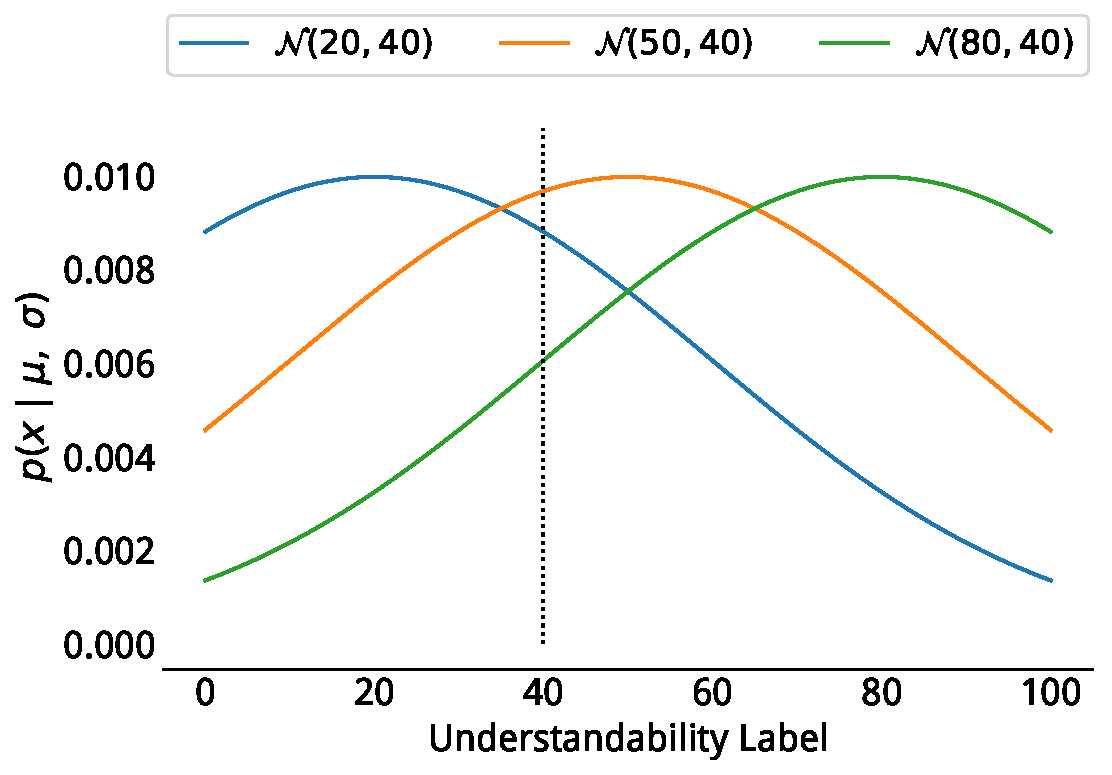
\includegraphics[width=0.8\textwidth]{figs/gaussians}
    \caption{Gaussian distribution for different $\mu$ values. A distribution with a higher $\mu$ generates higher understandability labels simulating that documents harder to read were retrieved. In the experiments in this Chapter, only documents with an understandability label lower than 40 are considered to easy-to-read, and therefore relevant in the understandability dimension.}
  \label{fig:gaussians}
\end{figure*}


We generated 1,000 runs for each topical relevance level and assessed the documents with different understandability labels generated by various Gaussian distributions. 
The results of different scenarios are shown in Table~\ref{tab:simulations}.
Each row of Table~\ref{tab:simulations} shows the results of simulations with different values for $T$, i.e., different expected number of relevant documents retrieved.
We varied the $\mu$ parameter of the Gaussian distributions employed to create the understandability labels. A smaller $\mu$ means that more understandable documents are retrieved.
In total fifteen experiments are shown in Table~\ref{tab:simulations}.

When increasing the expected number of relevant documents ($T$), Table~\ref{tab:simulations} shows that RBP increases. Likewise, uRBP increases, as it is bounded with topical relevance.
In turn, increasing $T$ has no effect on $RBP_u$, but increases $H_{RBP}$, as it directly depends on RBP.

When increasing the number of understandable documents retrieved (decreasing $\mu$), RBP stays constant, as it does not measure how understandable documents are.
uRBP, $RBP_u$ and $H_{RBP}$ increase.

We colored in blue and yellow an example that helps to illustrate the advantages of measuring each dimensions separately.
A system modification that aims to increase the understandability of the documents retrieved by an IR system might hurt the topical relevance of the documents retrieved by the system.
This situation could be translated in an initial system with results shown in blue in Table~\ref{tab:simulations} -- $T=0.6$ and $\mathcal{N}(40,40)$ -- 
becoming a system with results shown in yellow -- $T=0.5$ and $\mathcal{N}(30,40)$. 
Considering only RBP and uRBP, it is very hard to notice the gains in the understandability dimension: RBP decreases from 56 to 47 and uRBP decreases from 32 to 30.
However, when separately measuring $RBP_t$ (which is the same as RBP) and $RBP_u$, we can understand better what is happening with each dimension: $RBP_t$ decreases from 56 to 47, but $RBP_u$ increases from 49 to 60. Finally, $H_{RBP}$, which is giving the same importance to both dimensions, shows that, although very different, both system are equivalent. If document topicality is more important than document understandability, the weights of each dimension can be tweaked in the harmonic mean formula, exactly as precision and recall are balanced in the $F$ formula.

%The drawback of separating the evaluation of each dimension before merging them with an harmonic mean is that a clear 

\begin{table*}
\centering \caption{We varied $T$, the expected number of topical relevance (rows), and the mean $\mu$ of Gaussian distribution used to generate understandability labels (columns). 
    A smaller $\mu$ means that easier to read documents are retrieved.
    We showed the average and standard deviation of each experiment. All numbers were multiplied by 100. }
\label{tab:simulations} \resizebox{1.\textwidth}{!}{ %
\begin{tabular}{cllllllllllll}
\toprule 
\multirow{2}{*}{$T$}  & \multicolumn{4}{c}{\textbf{Understandability $\mathcal{N}$(50,40)}} & \multicolumn{4}{c}{\textbf{Understandability $\mathcal{N}$(40,40)}} & \multicolumn{4}{c}{\textbf{Understandability $\mathcal{N}$(30,40)}}\tabularnewline
\cmidrule{2-13}
 & RBP  & uRBP  & $RBP_{u}$  & $H_{RBP}$  & RBP  & uRBP  & $RBP_{u}$  & $H_{RBP}$  & RBP  & uRBP  & $RBP_{u}$  & $H_{RBP}$ \tabularnewline
\midrule 
0.3 & 28$\pm$1 & 14$\pm$1 & 41$\pm$1 & 30$\pm$1 & 28$\pm$1 & 16$\pm$1 & 50$\pm$1 & 33$\pm$1 & 28$\pm$1 & 19$\pm$1 & 59$\pm$2 & 35$\pm$1\tabularnewline
0.4 & 38$\pm$2 & 19$\pm$1 & 41$\pm$1 & 36$\pm$1 & 38$\pm$2 & 21$\pm$1 & 50$\pm$1 & 39$\pm$1 & 38$\pm$2 & 25$\pm$1 & 60$\pm$1 & 43$\pm$1\tabularnewline
0.5 & 47$\pm$1 & 24$\pm$1 & 41$\pm$1 & 40$\pm$1 & 47$\pm$1 & 26$\pm$1 & 49$\pm$1 & 45$\pm$1 & {\cellcolor{yellow!25}} 47$\pm$1 & {\cellcolor{yellow!25}} 30$\pm$1 & {\cellcolor{yellow!25}} 60$\pm$1 & {\cellcolor{yellow!25}} 49$\pm$1\tabularnewline
0.6 & 56$\pm$1 & 28$\pm$1 & 41$\pm$1 & 44$\pm$1 & {\cellcolor{blue!25}}56$\pm$1 & {\cellcolor{blue!25}}32$\pm$1 &  {\cellcolor{blue!25}}49$\pm$2 & {\cellcolor{blue!25}}49$\pm$1 & 56$\pm$1 & 37$\pm$1 & 60$\pm$1 & 55$\pm$1\tabularnewline
0.7 & 65$\pm$1 & 33$\pm$1 & 42$\pm$1 & 48$\pm$1 & 65$\pm$1 & 37$\pm$1 & 49$\pm$1 & 53$\pm$1 & 65$\pm$1 & 42$\pm$1 & 60$\pm$1 & 60$\pm$1\tabularnewline
\bottomrule
\end{tabular}} 
\end{table*}


 

%%%%%%%%%%%%%%%%%%%%%%%%%%%%%%%%%%%%%%%%%%%%%%%%%%%%%%%%%%%%%%%%%%%%%%%%%%%%%%%%%%%%%%%%%%%%%%%%%%%%%%%%%%%%%%%%%%%%%%%%%%%%%%%%
%%%%%%%%%%%%%%%%%%%%%%%%%%%%%%%%%%%%%%%%%%%%%%%%%%%%%%%%%%%%%%%%%%%%%%%%%%%%%%%%%%%%%%%%%%%%%%%%%%%%%%%%%%%%%%%%%%%%%%%%%%%%%%%%
%%%%%%%%%%%%%%%%%%%%%%%%%%%%%%%%%%%%%%%%%%%%%%%%%%%%%%%%%%%%%%%%%%%%%%%%%%%%%%%%%%%%%%%%%%%%%%%%%%%%%%%%%%%%%%%%%%%%%%%%%%%%%%%%
%%%%%%%%%%%%%%%%%%%%%%%%%%%%%%%%%%%%%%%%%%%%%%%%%%%%%%%%%%%%%%%%%%%%%%%%%%%%%%%%%%%%%%%%%%%%%%%%%%%%%%%%%%%%%%%%%%%%%%%%%%%%%%%%

